%! TEX root = ../main.tex
\documentclass[main]{subfiles}

\begin{document}

\section{表面繊維}

まず,カーリングブラシパッドの汚れが多い箇所をFig.\ref{fig:1},Fig.\ref{fig:2},Fig.\ref{fig:3},
Fig.\ref{fig:4},Fig.\ref{fig:5}に示す.


\begin{figure}[H]
    \centering
    \begin{subfigure}[htbp]{0.45\linewidth}
        \centering
        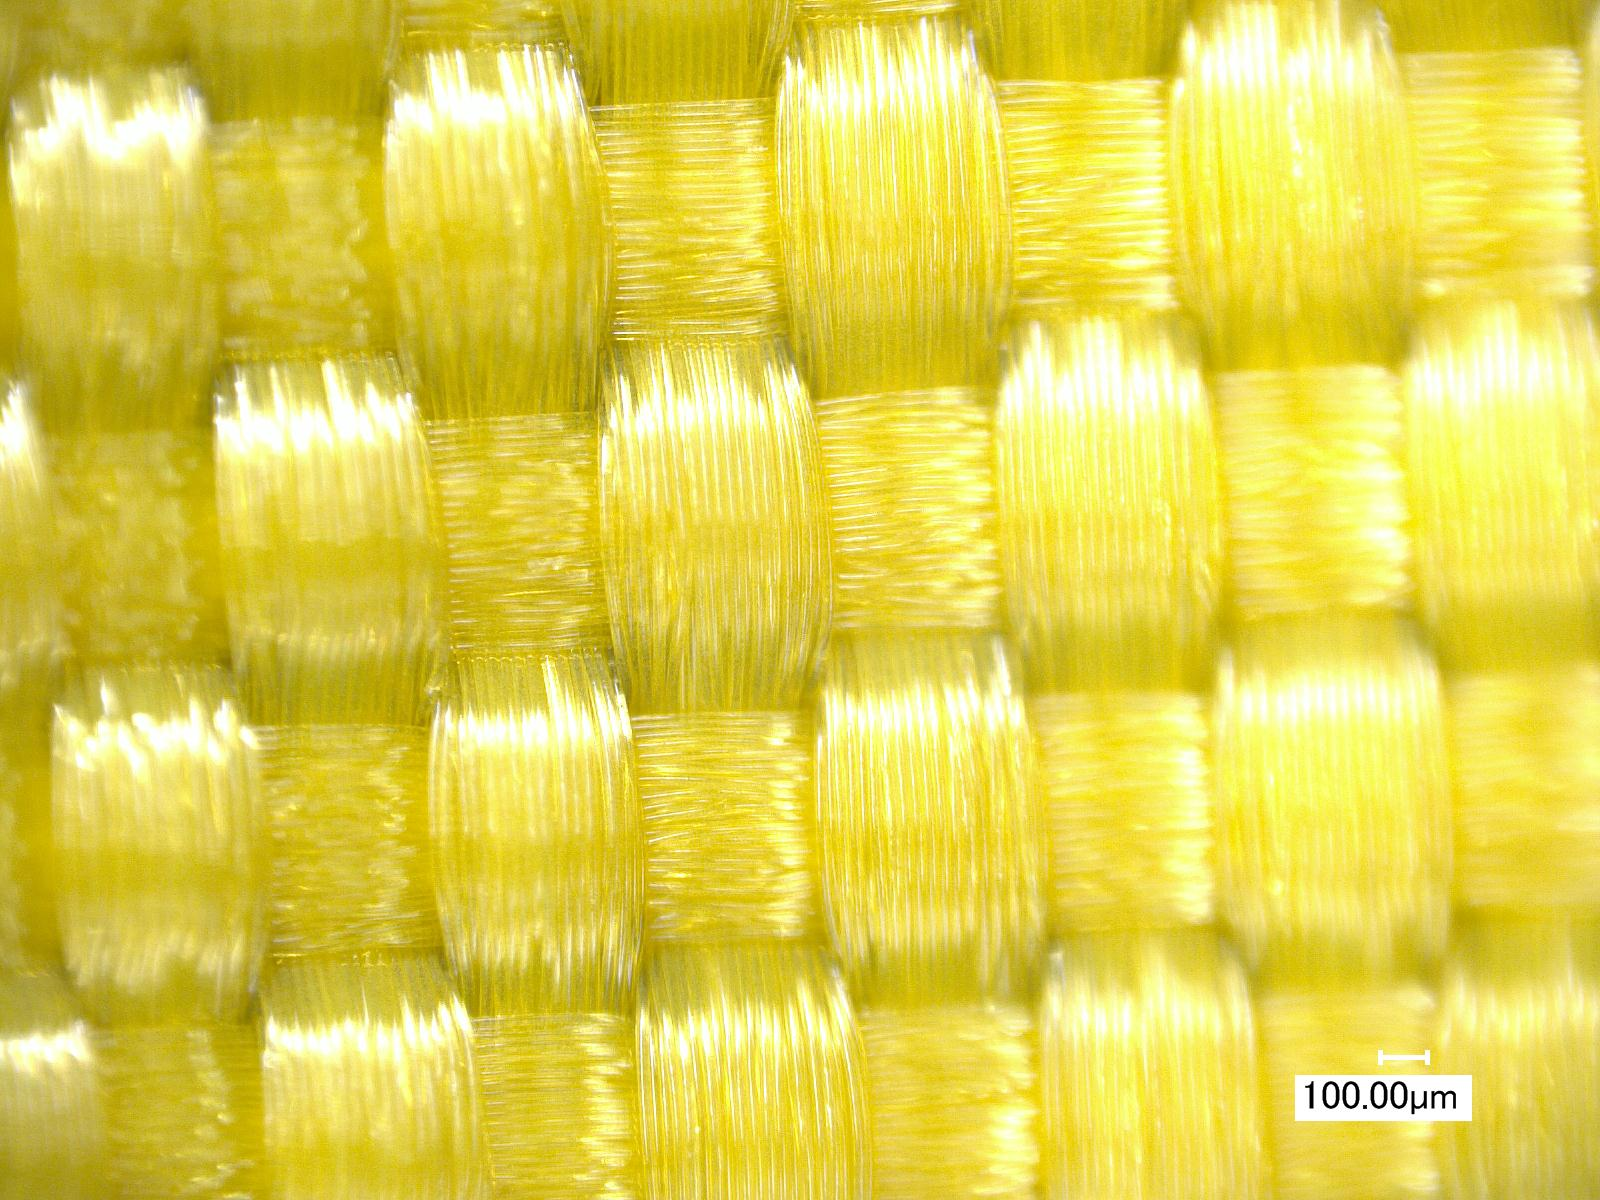
\includegraphics[keepaspectratio, width=0.8\linewidth]{figures/縁/カーリングパッド未使用低倍率.jpg}
        \caption{低倍率(100倍)}
        \label{fig:label}
    \end{subfigure}
    \begin{subfigure}[htbp]{0.45\linewidth}
        \centering
        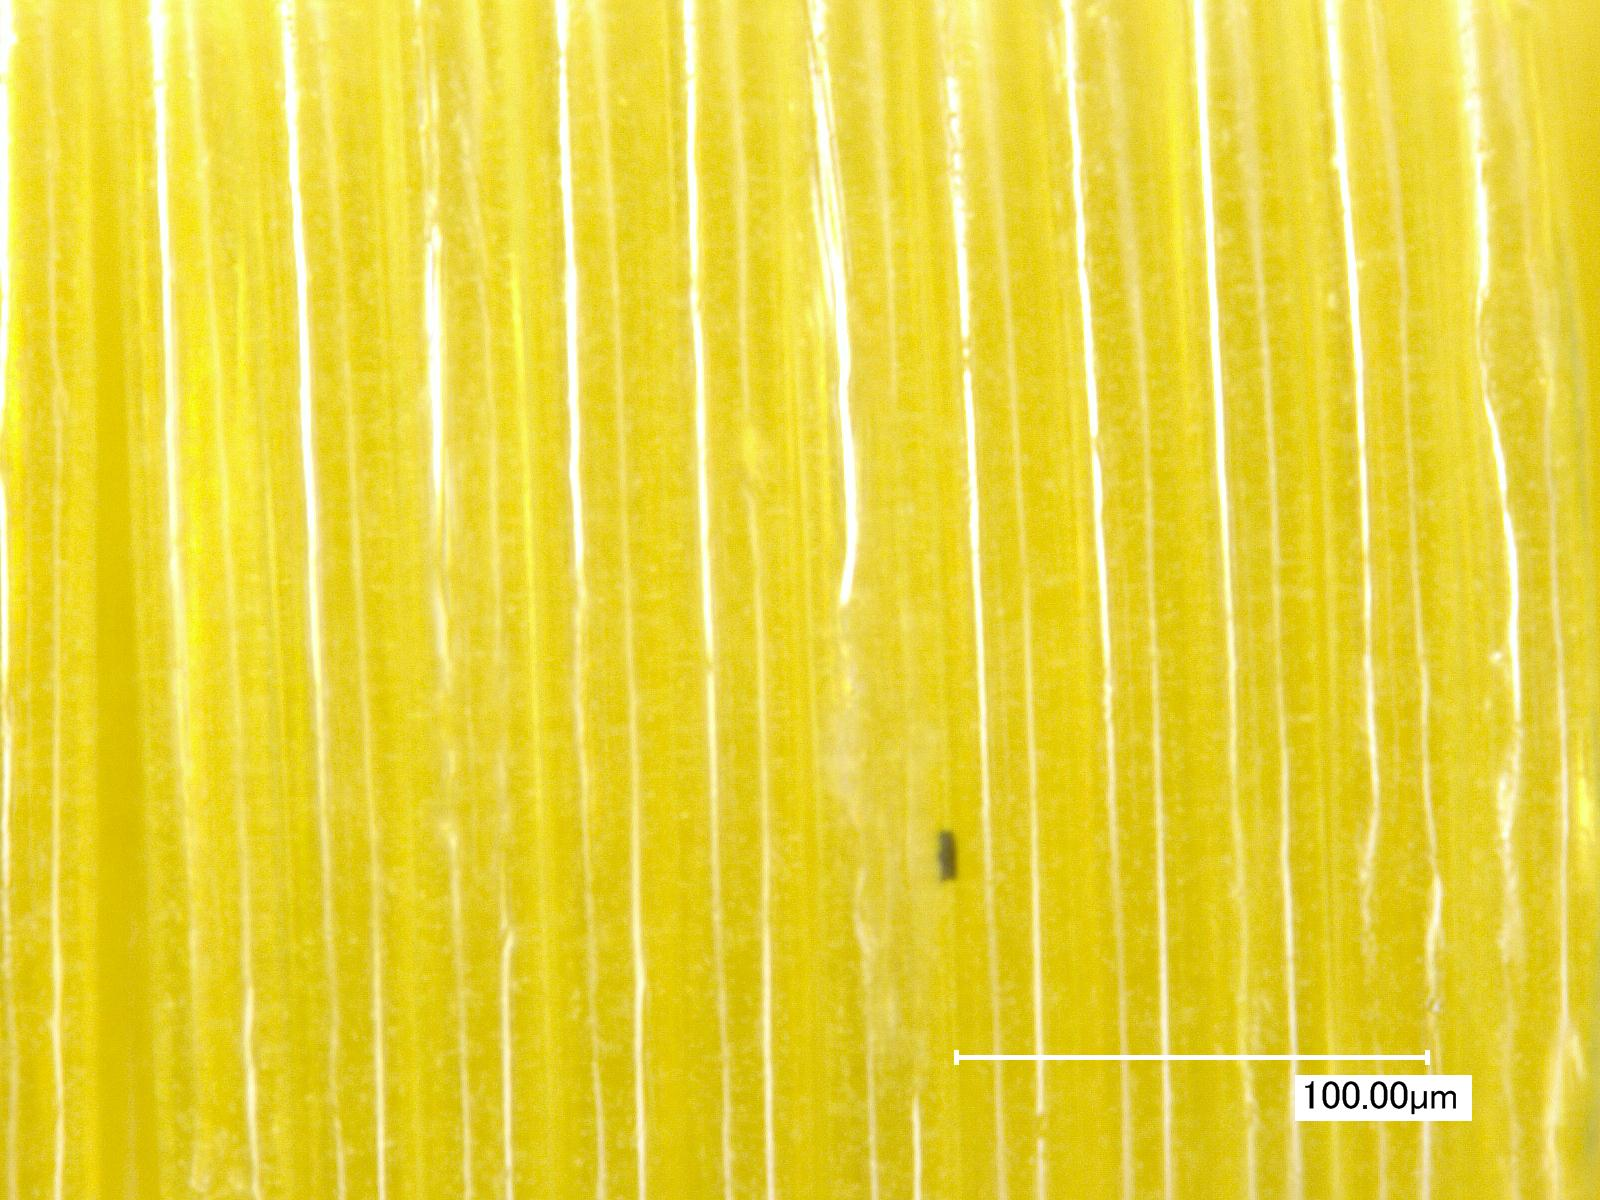
\includegraphics[keepaspectratio, width=0.8\linewidth]{figures/縁/カーリングパッド未使用.jpg}
        \caption{高倍率(1000倍)}
        \label{fig:label}
    \end{subfigure}
    \caption{未使用}
    \label{fig:1}
\end{figure}

\begin{figure}[H]
    \centering
    \begin{subfigure}[htbp]{0.45\linewidth}
        \centering
        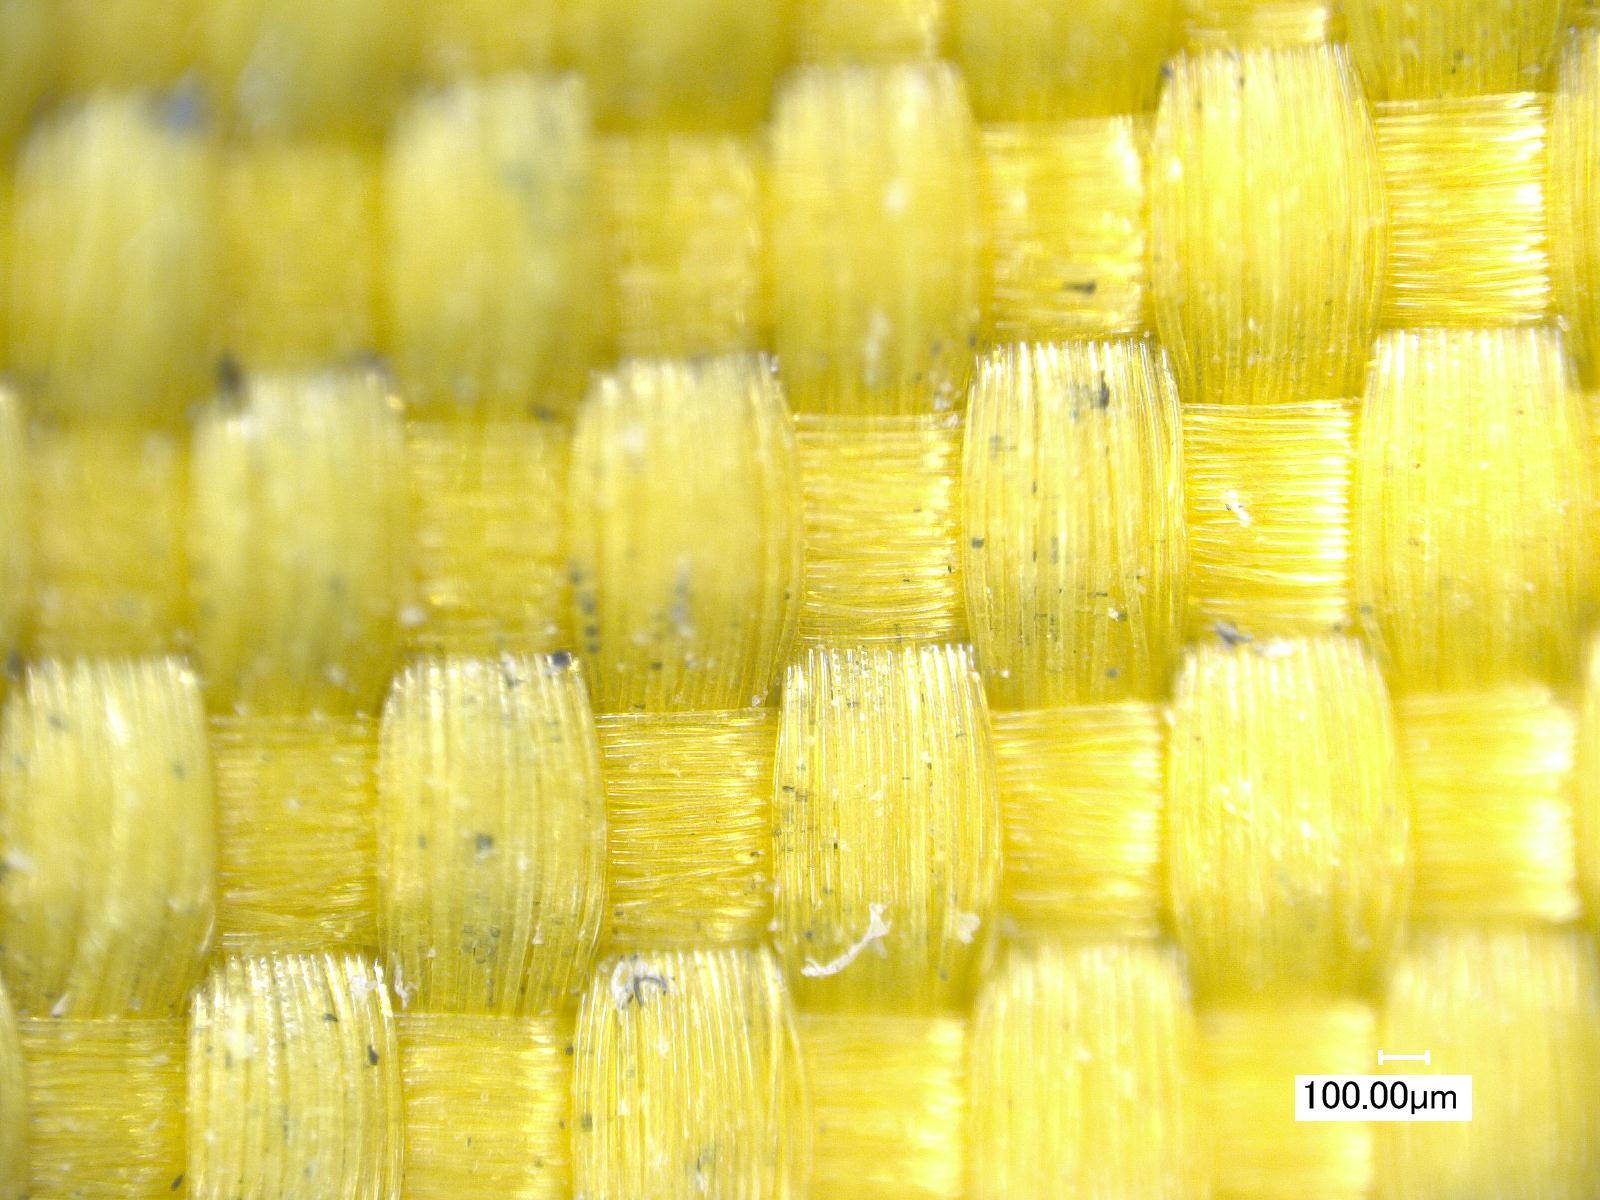
\includegraphics[keepaspectratio, width=0.8\linewidth]{figures/縁/カーリングパッド10-15低倍率.jpg}
        \caption{低倍率(100倍)}
        \label{fig:label}
    \end{subfigure}
    \begin{subfigure}[htbp]{0.45\linewidth}
        \centering
        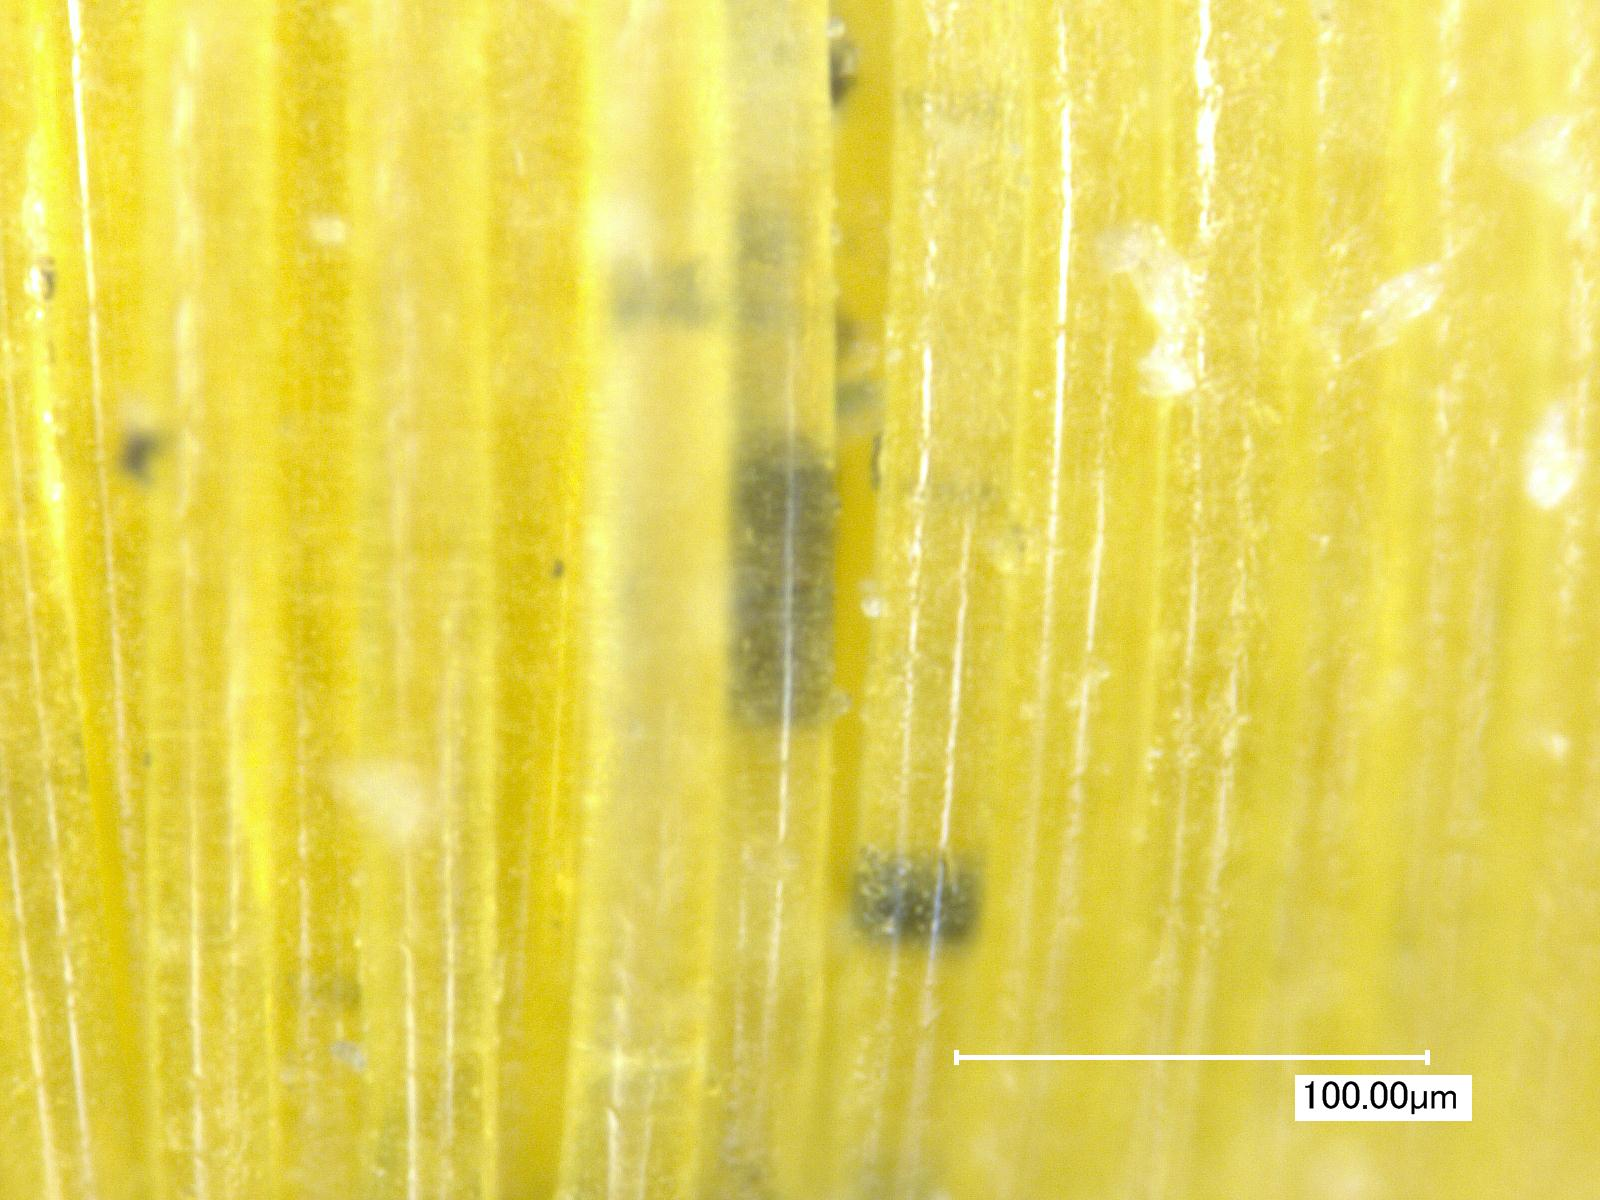
\includegraphics[keepaspectratio, width=0.8\linewidth]{figures/縁/カーリングパッド10-15.jpg}
        \caption{高倍率(1000倍)}
        \label{fig:label}
    \end{subfigure}
    \caption{10~15投使用A(汚れの偏りなし)}
    \label{fig:2}
\end{figure}
    

\begin{figure}[H]
    \centering
    \begin{subfigure}[htbp]{0.45\linewidth}
        \centering
        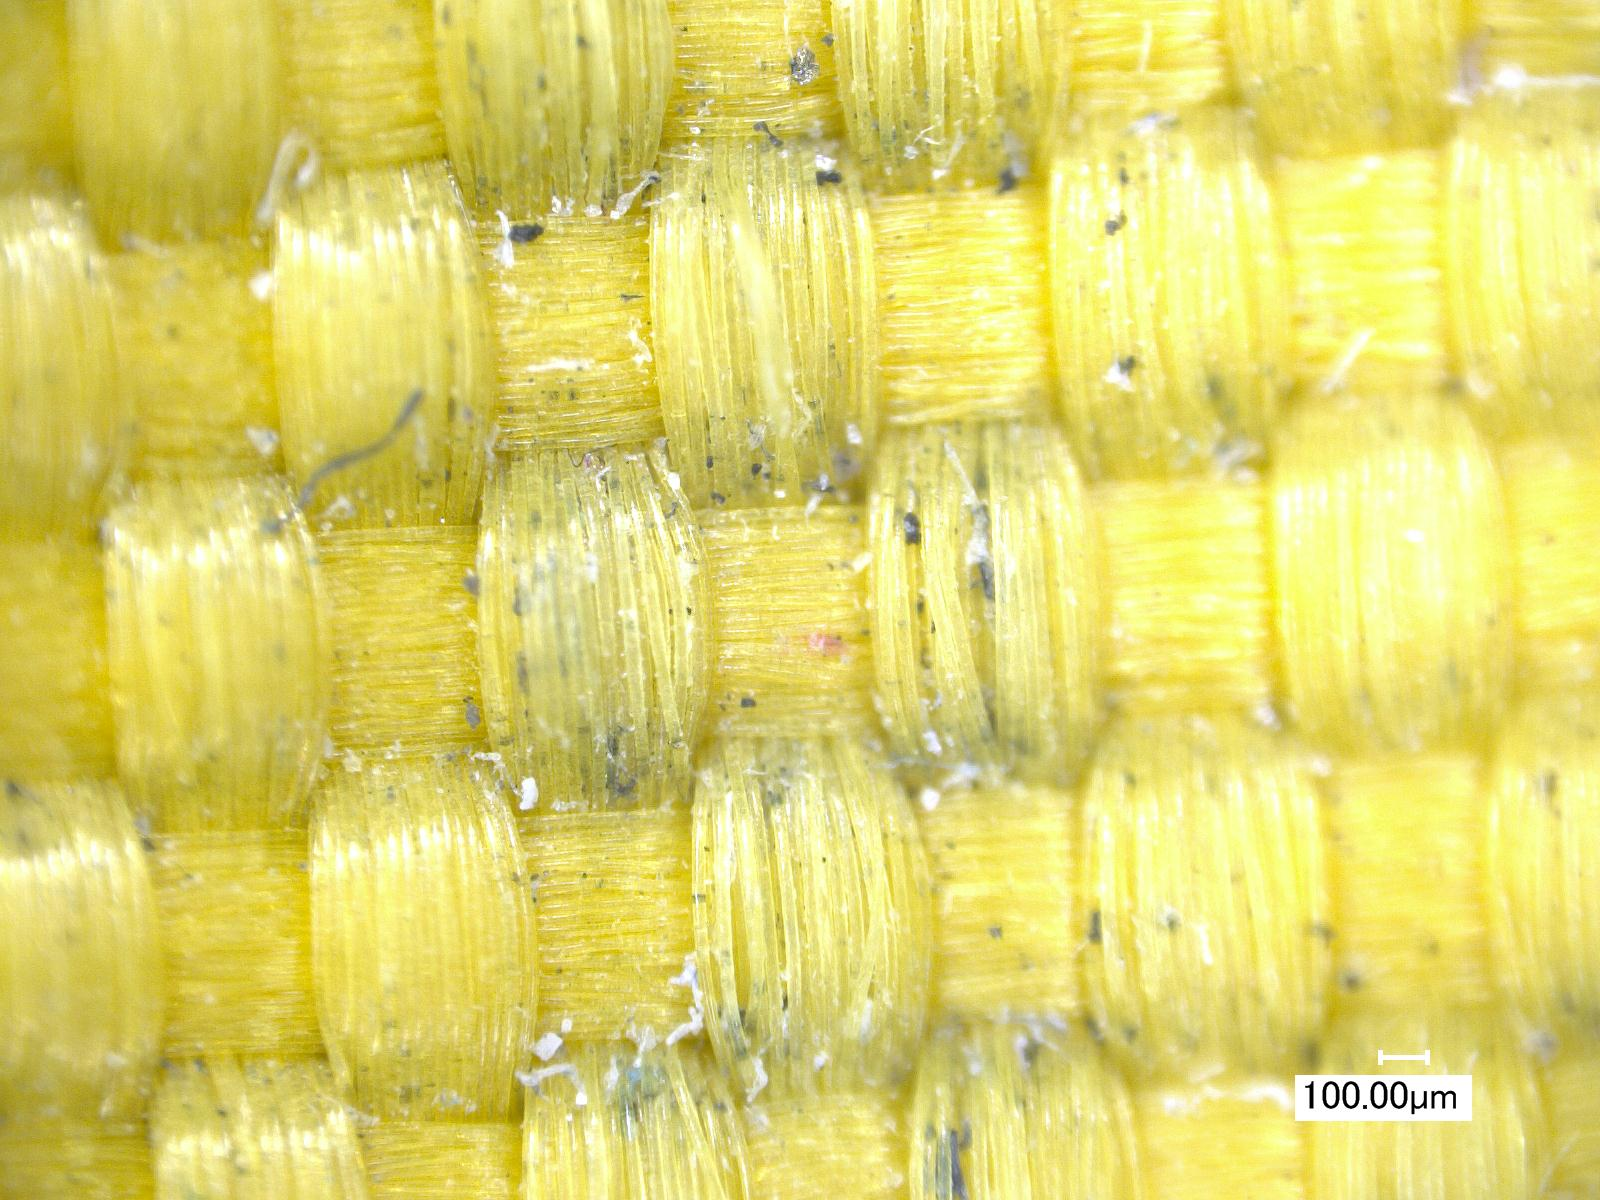
\includegraphics[keepaspectratio, width=0.8\linewidth]{figures/縁/カーリングパッド10-15低倍率B.jpg}
        \caption{低倍率(100倍)}
        \label{fig:label}
    \end{subfigure}
    \begin{subfigure}[htbp]{0.45\linewidth}
        \centering
        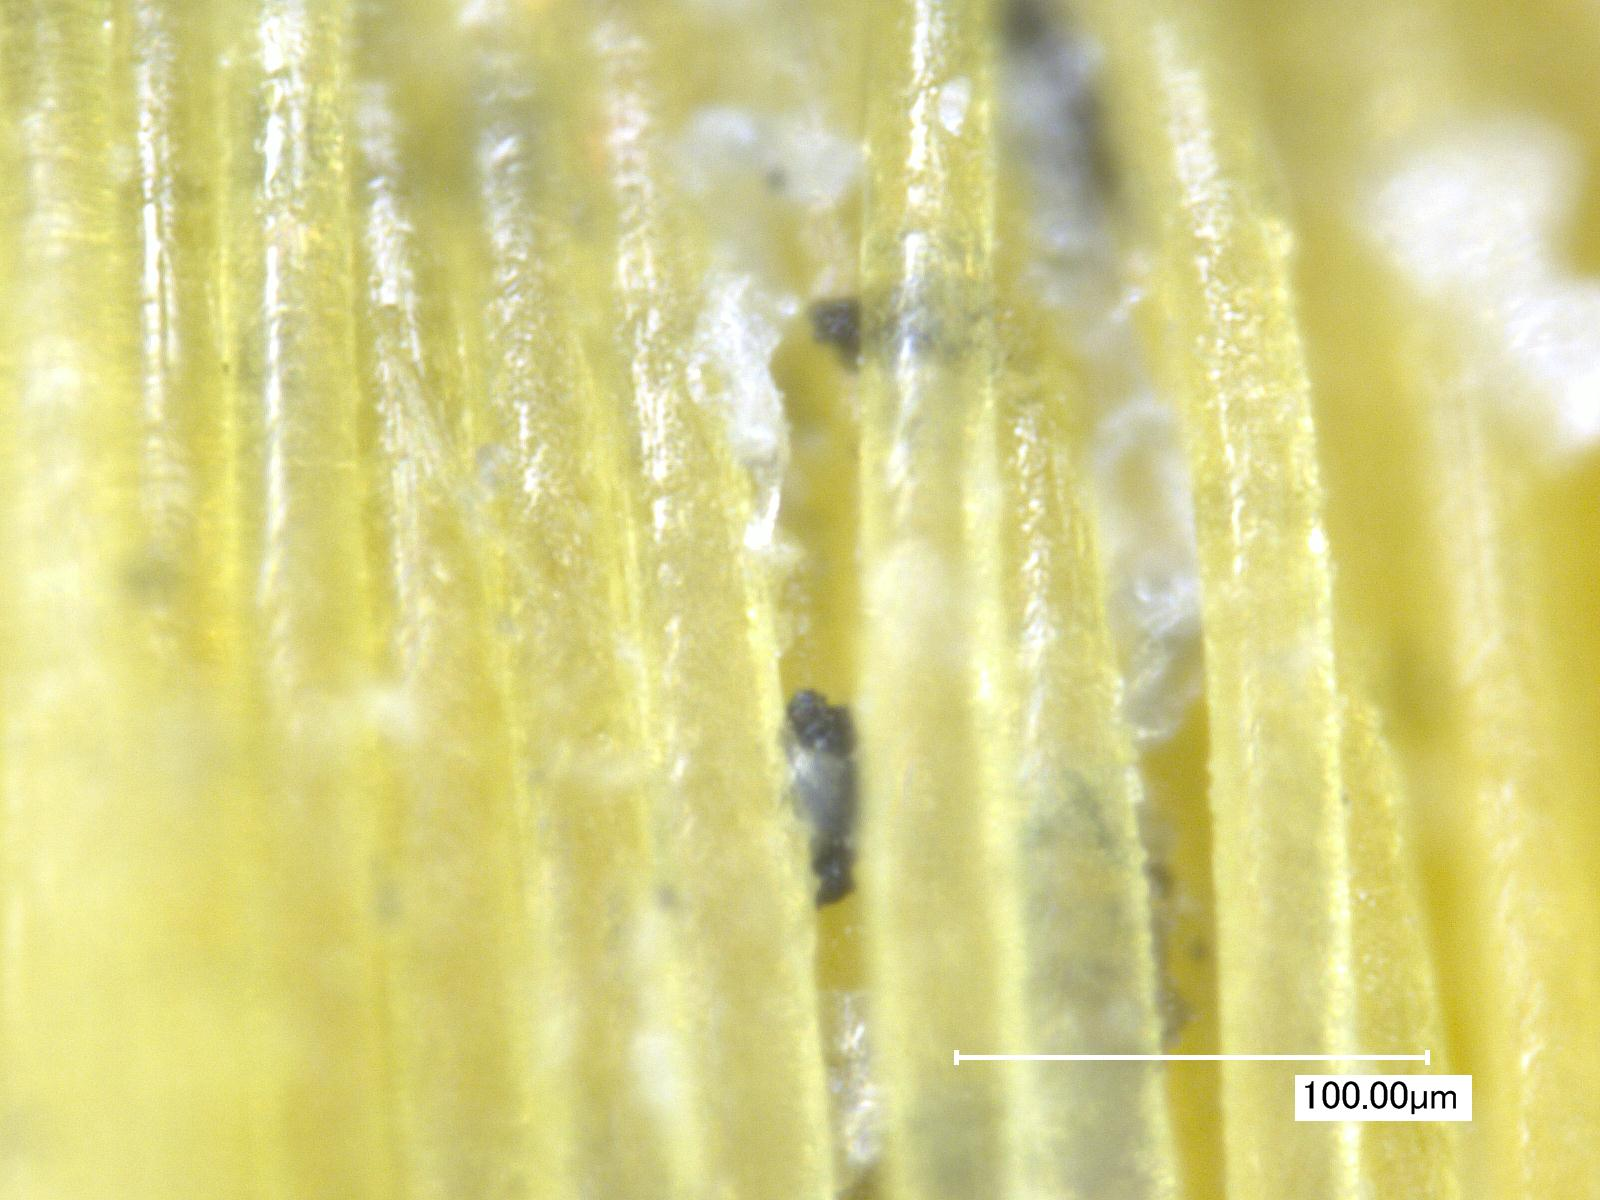
\includegraphics[keepaspectratio, width=0.8\linewidth]{figures/縁/カーリングパッド10-15B.jpg}
        \caption{高倍率(1000倍)}
        \label{fig:label}
    \end{subfigure}
    \caption{10~15投使用B(汚れの偏りあり)}
    \label{fig:3}
\end{figure}

\begin{figure}[H]
    \centering
    \begin{subfigure}[htbp]{0.45\linewidth}
        \centering
        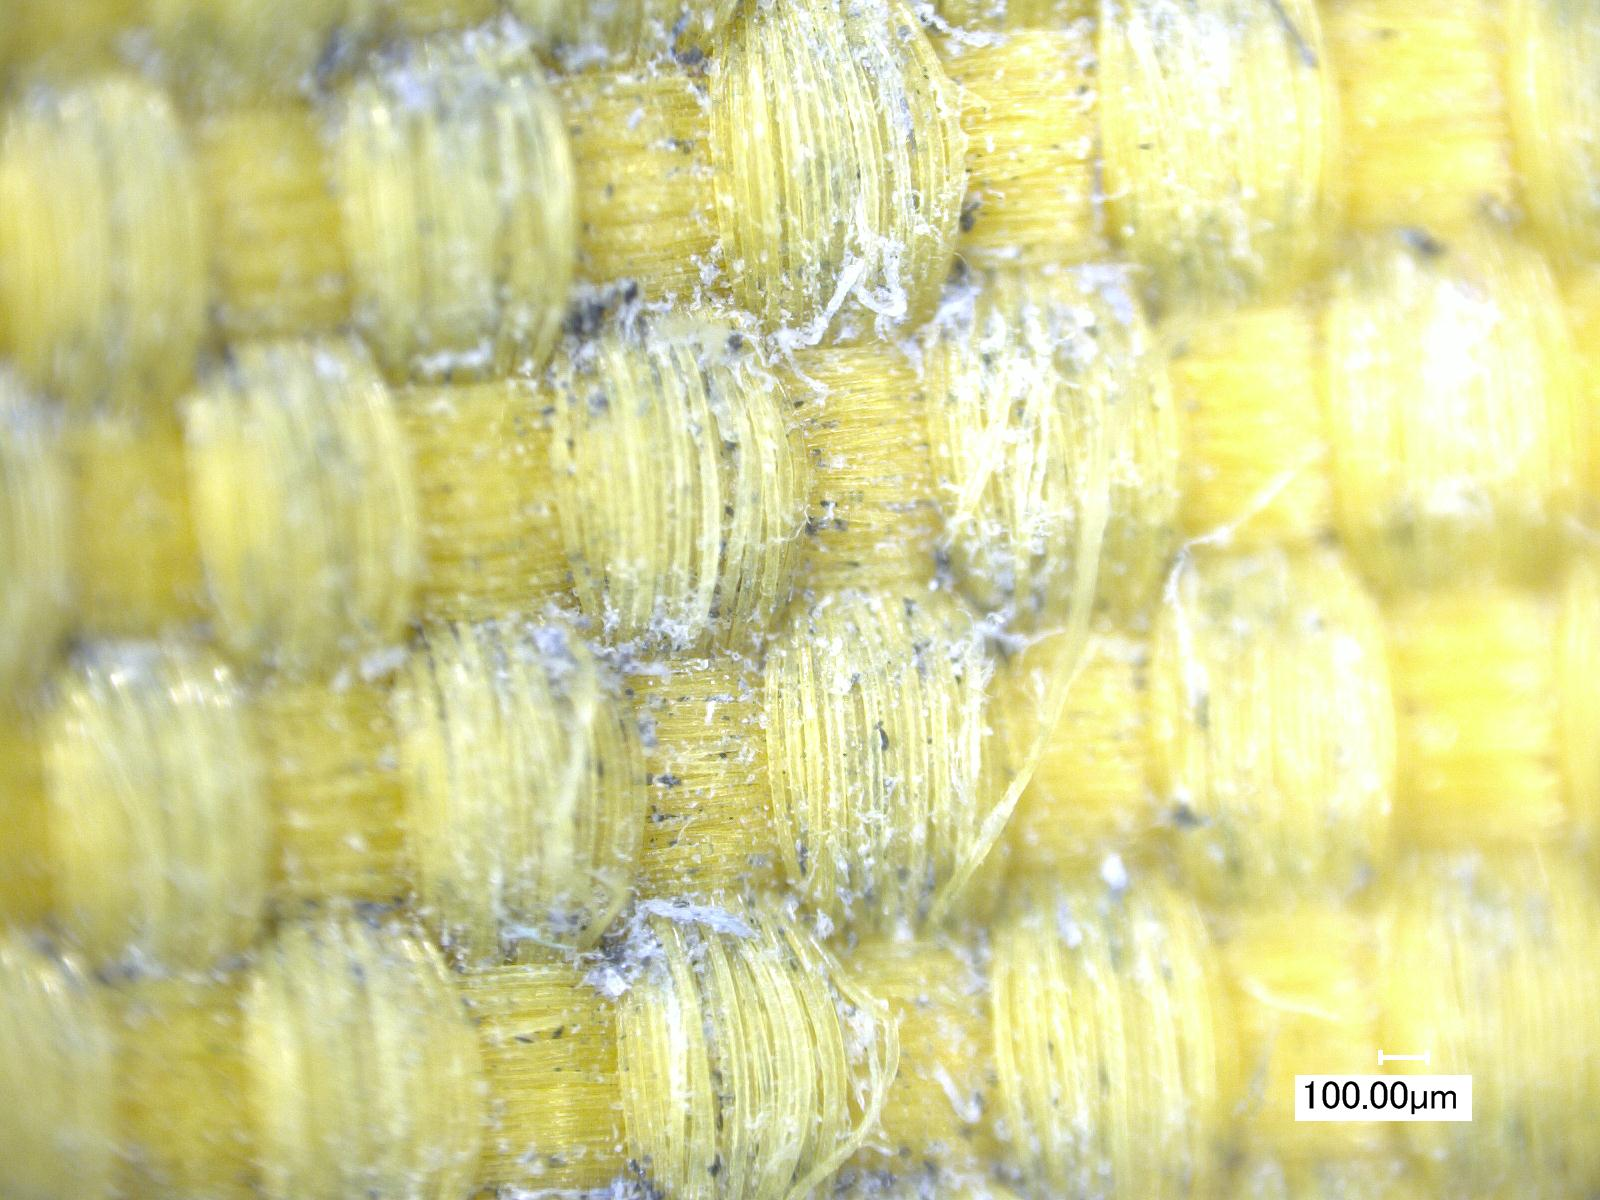
\includegraphics[keepaspectratio, width=0.8\linewidth]{figures/縁/カーリングパッド長期低倍率.jpg}
        \caption{低倍率(100倍)}
        \label{fig:label}
    \end{subfigure}
    \begin{subfigure}[htbp]{0.45\linewidth}
        \centering
        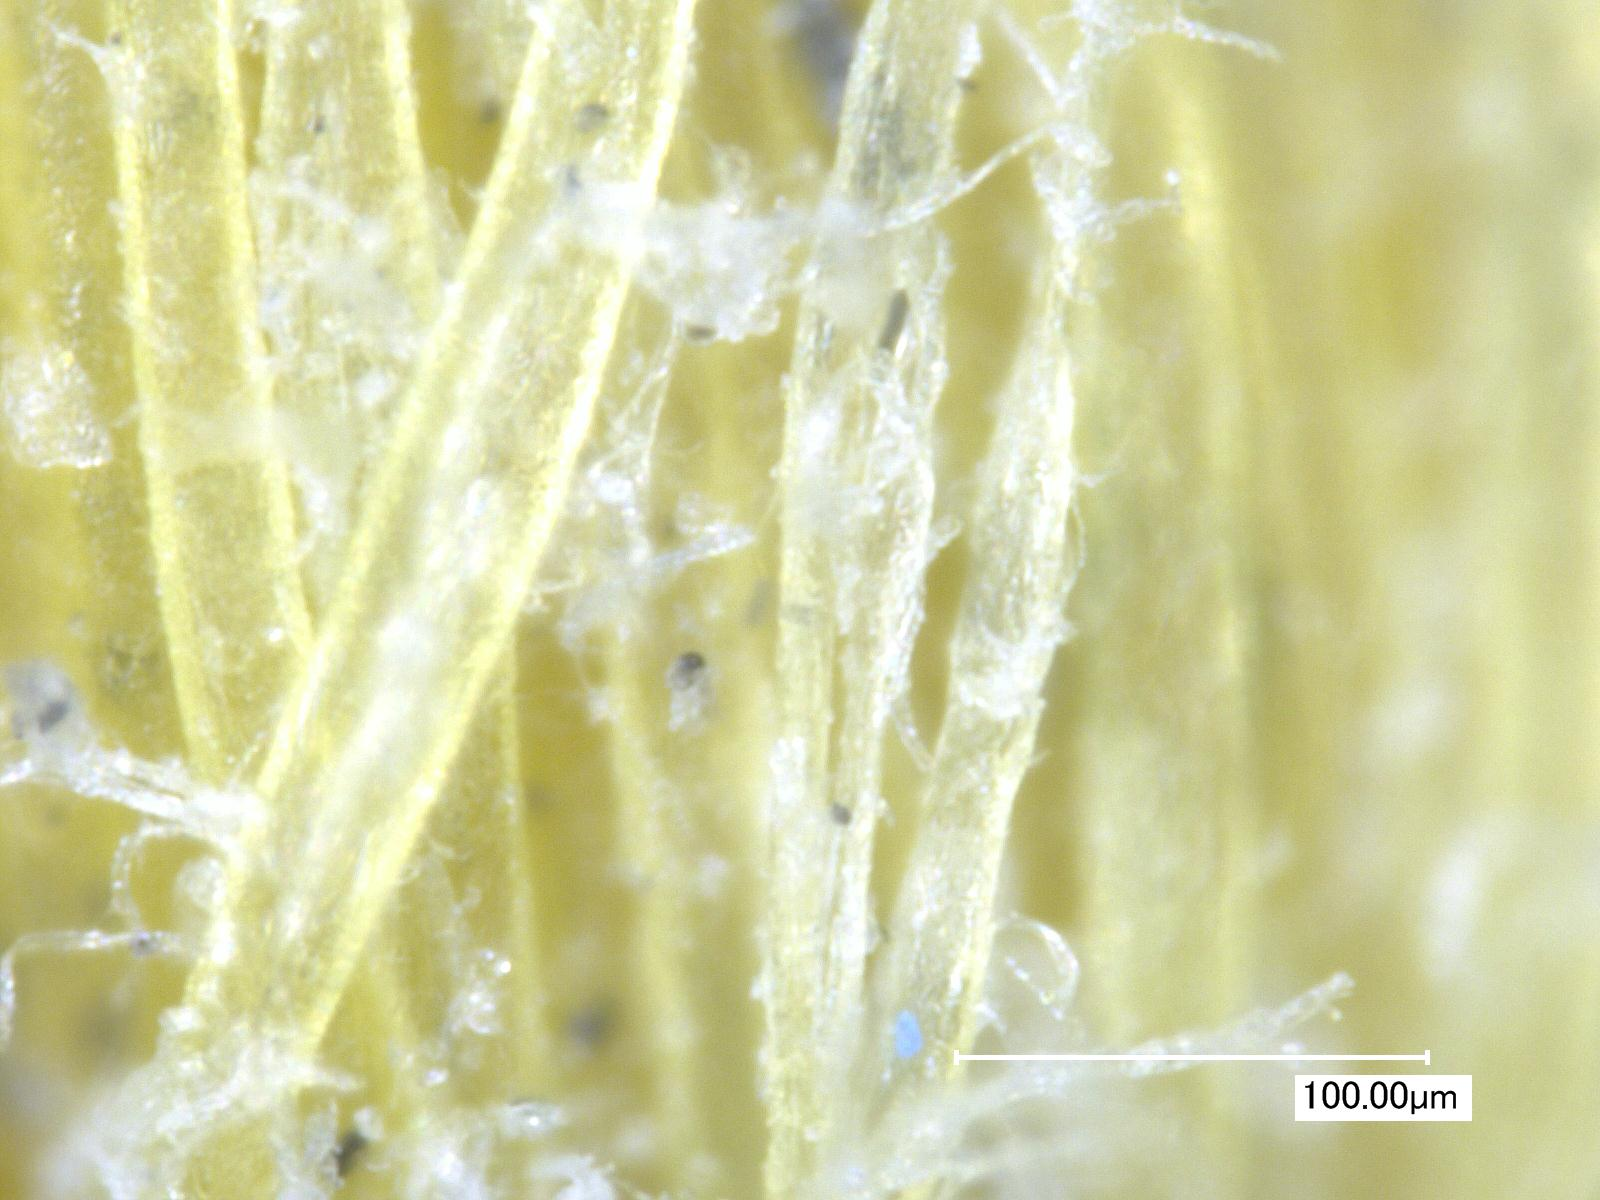
\includegraphics[keepaspectratio, width=0.8\linewidth]{figures/縁/カーリングパッド長期.jpg}
        \caption{高倍率(1000倍)}
        \label{fig:label}
    \end{subfigure}
    \caption{長期間使用サンプルA}
    \label{fig:4}
\end{figure}
    
\begin{figure}[H]
    \centering
    \begin{subfigure}[htbp]{0.45\linewidth}
        \centering
        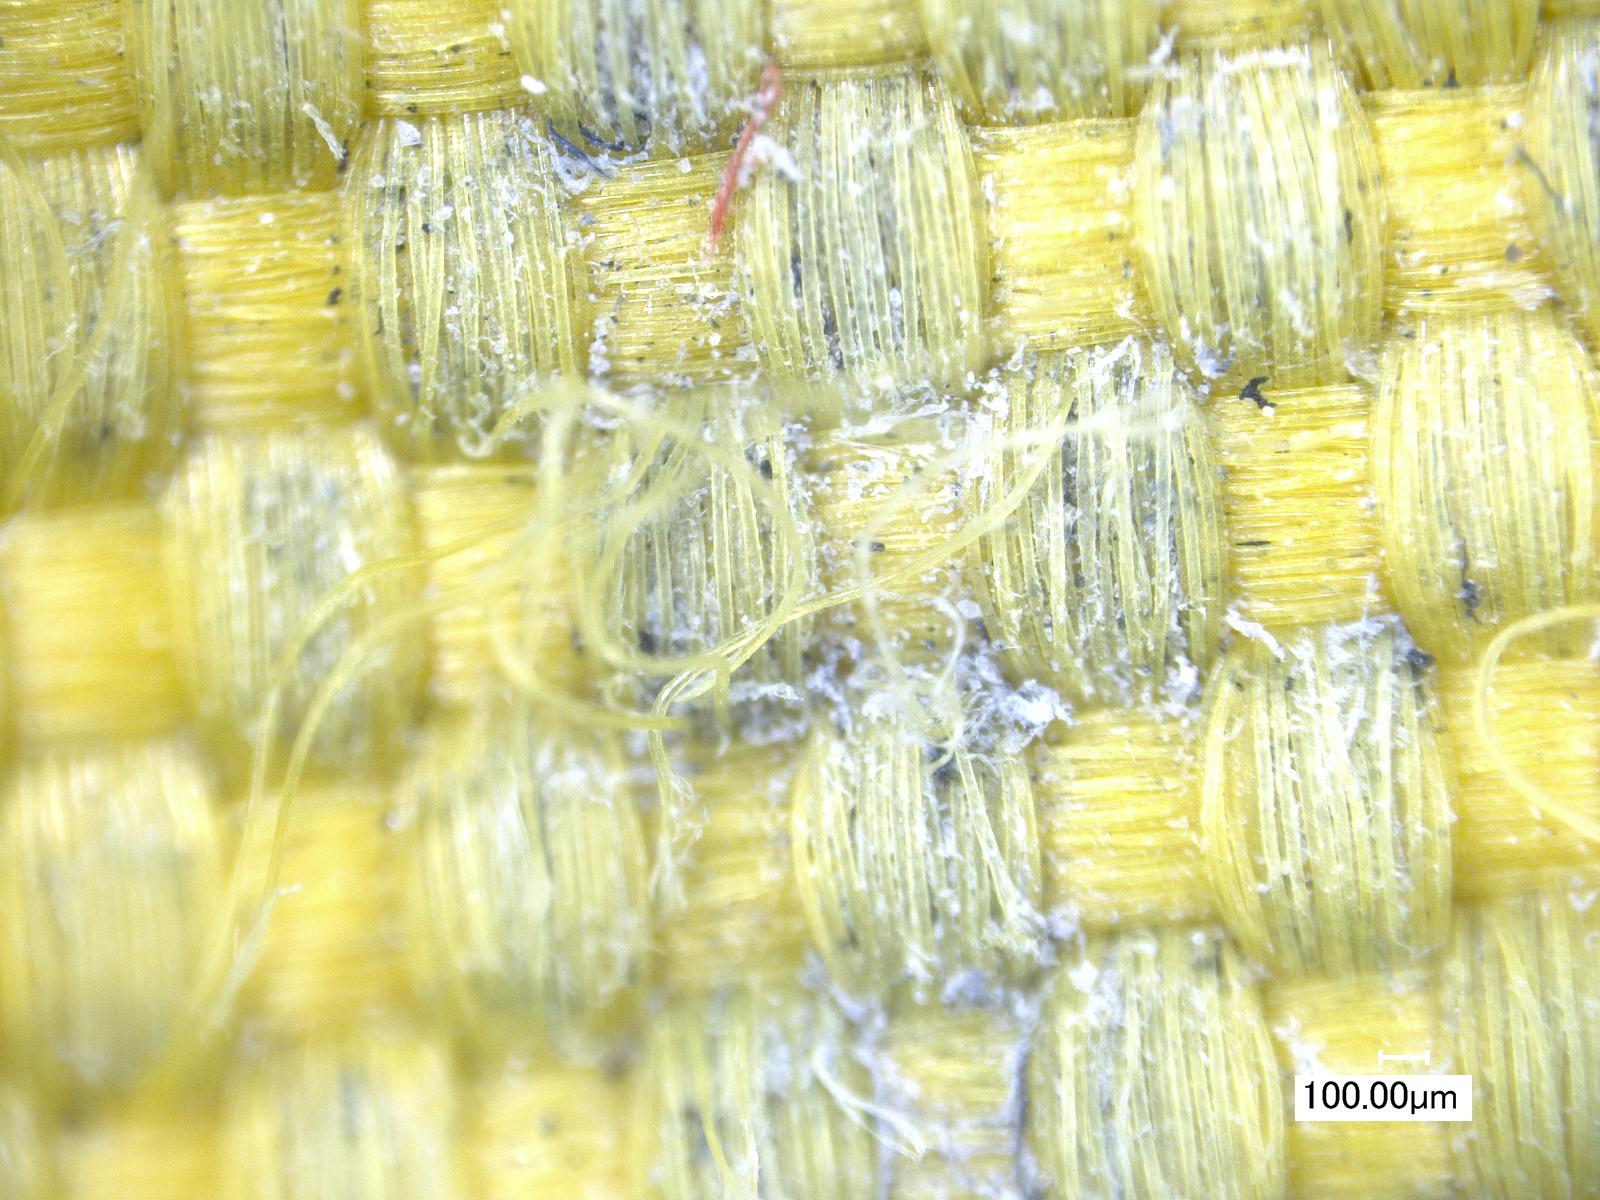
\includegraphics[keepaspectratio, width=0.8\linewidth]{figures/縁/カーリングパッド長期低倍率B.jpg}
        \caption{低倍率(100倍)}
        \label{fig:label}
    \end{subfigure}
    \begin{subfigure}[htbp]{0.45\linewidth}
        \centering
        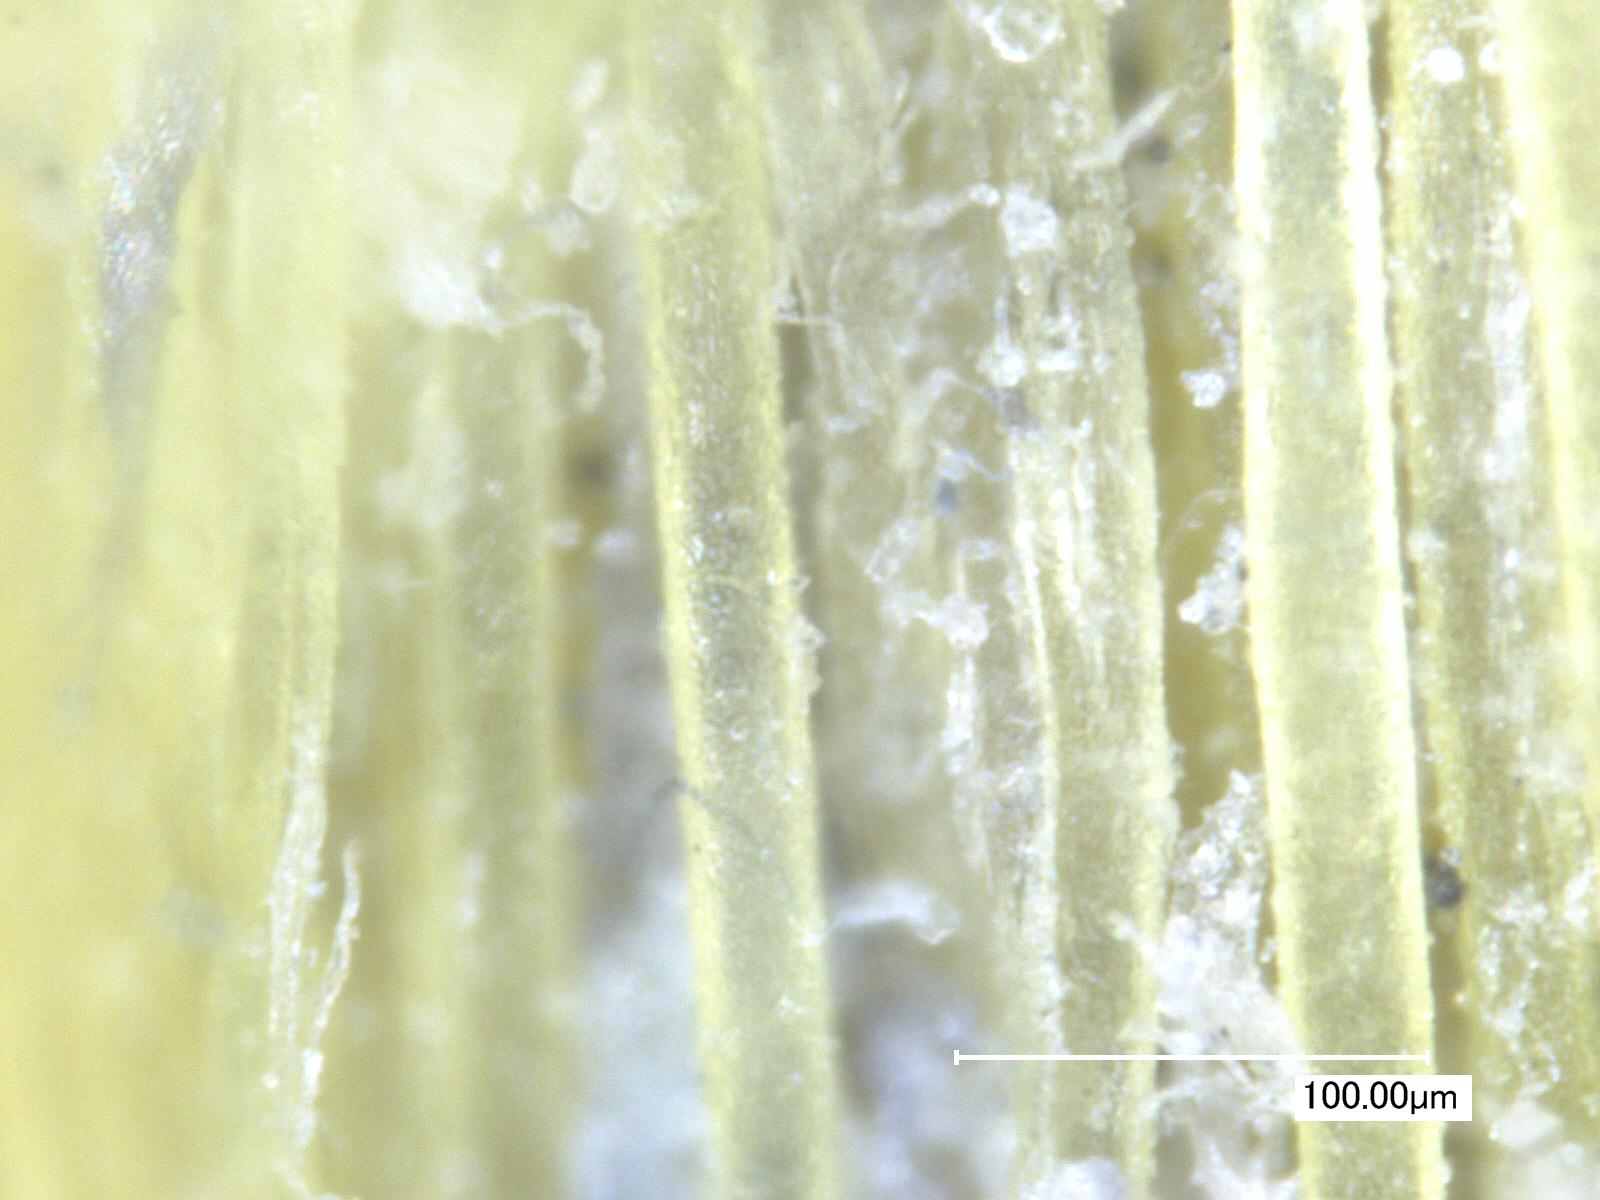
\includegraphics[keepaspectratio, width=0.8\linewidth]{figures/縁/カーリングパッド長期B.jpg}
        \caption{高倍率(1000倍)}
        \label{fig:label}
    \end{subfigure}
    \caption{長期間使用サンプルB}
    \label{fig:5}
\end{figure}

低倍率で比較した際に,スイープ方向に垂直に並んでいる繊維に違いがみられたので,その箇所を高倍率で観察した.
未使用のものは1本1本の繊維が隙間なく並んでいた.
それに対して,10~15投使用したものは隙間が増えていた.
長期間使用したものに関しては,繊維が切れているものもあった.
10~15投使用したものは2つのサンプルで摩耗具合に差があった.
また,使用回数が多くなるほどゴミの付着量が多い.

次にカーリングブラシパッドのそれぞれのサンプルで汚れの少ない箇所の結果をFig.\ref{fig:6},Fig.\ref{fig:7}に示す.



\begin{figure}[H]
    \centering
    \begin{subfigure}[htbp]{0.45\linewidth}
        \centering
        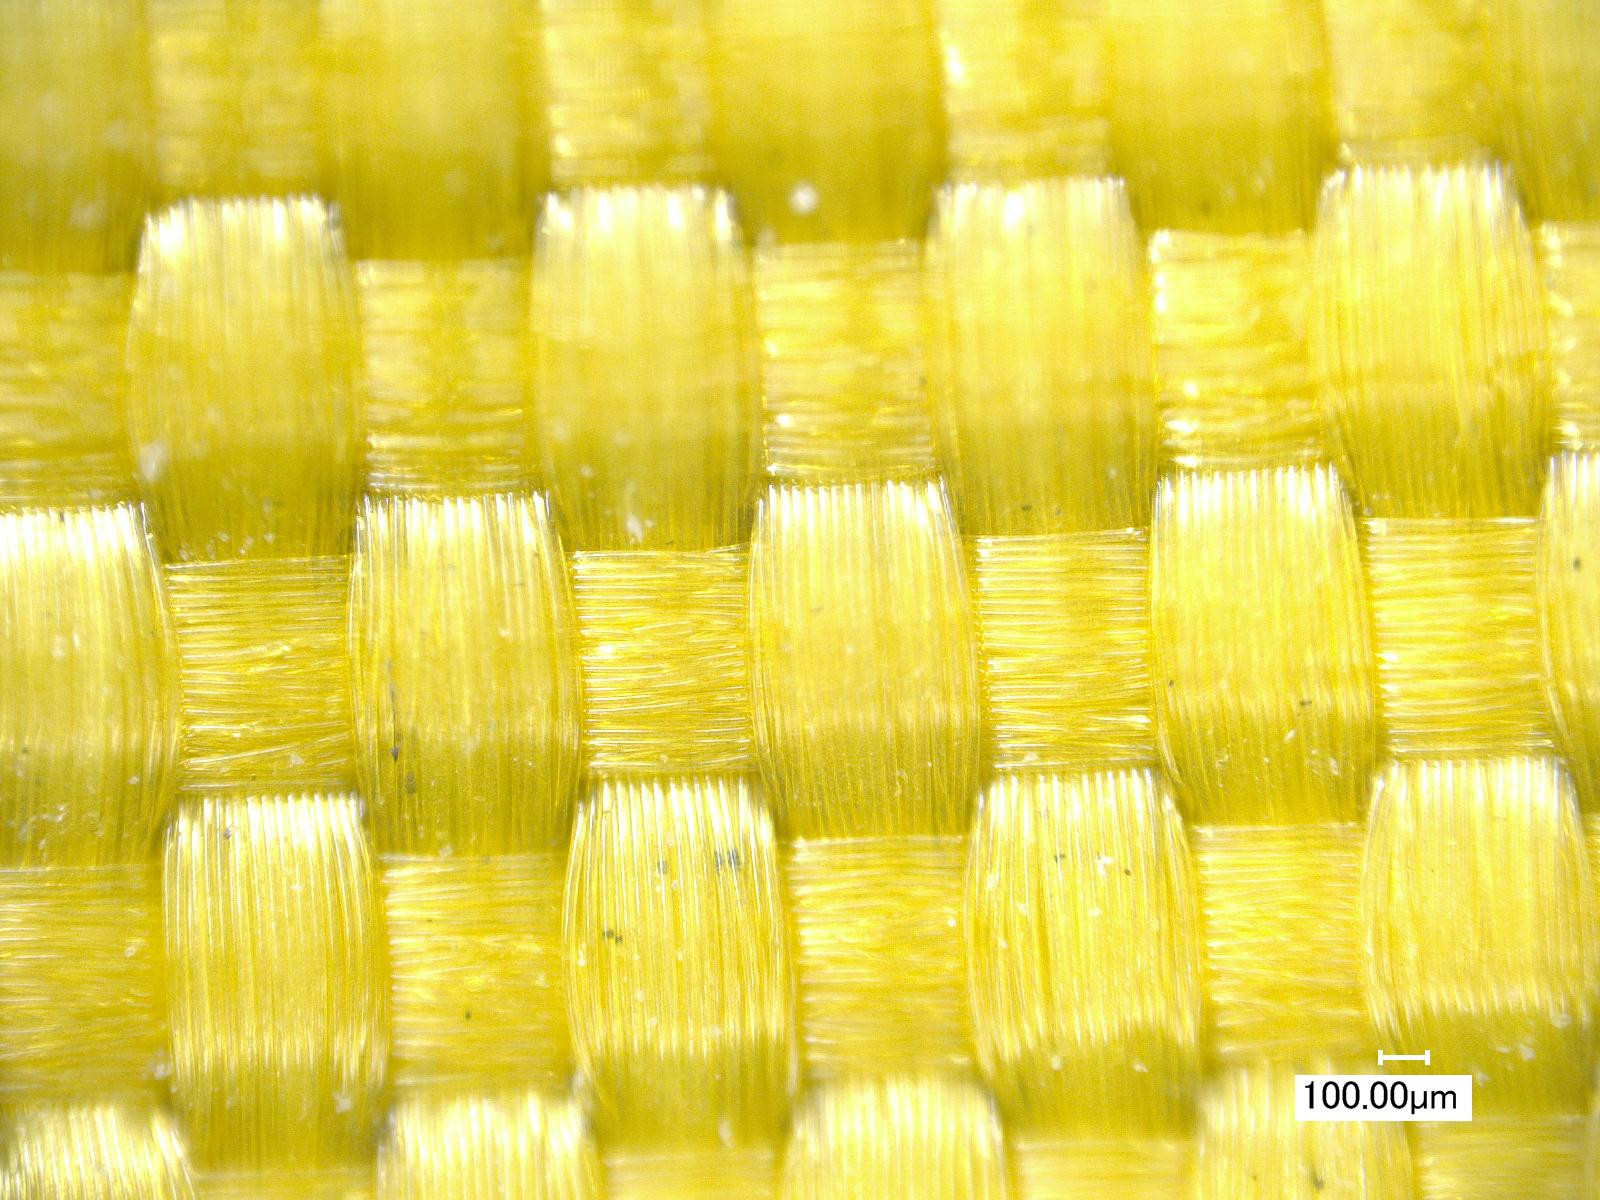
\includegraphics[keepaspectratio, width=0.8\linewidth]{figures/中心/カーリングパッド10-15低倍率.jpg}
        \caption{低倍率(100倍)}
        \label{fig:label}
    \end{subfigure}
    \begin{subfigure}[htbp]{0.45\linewidth}
        \centering
        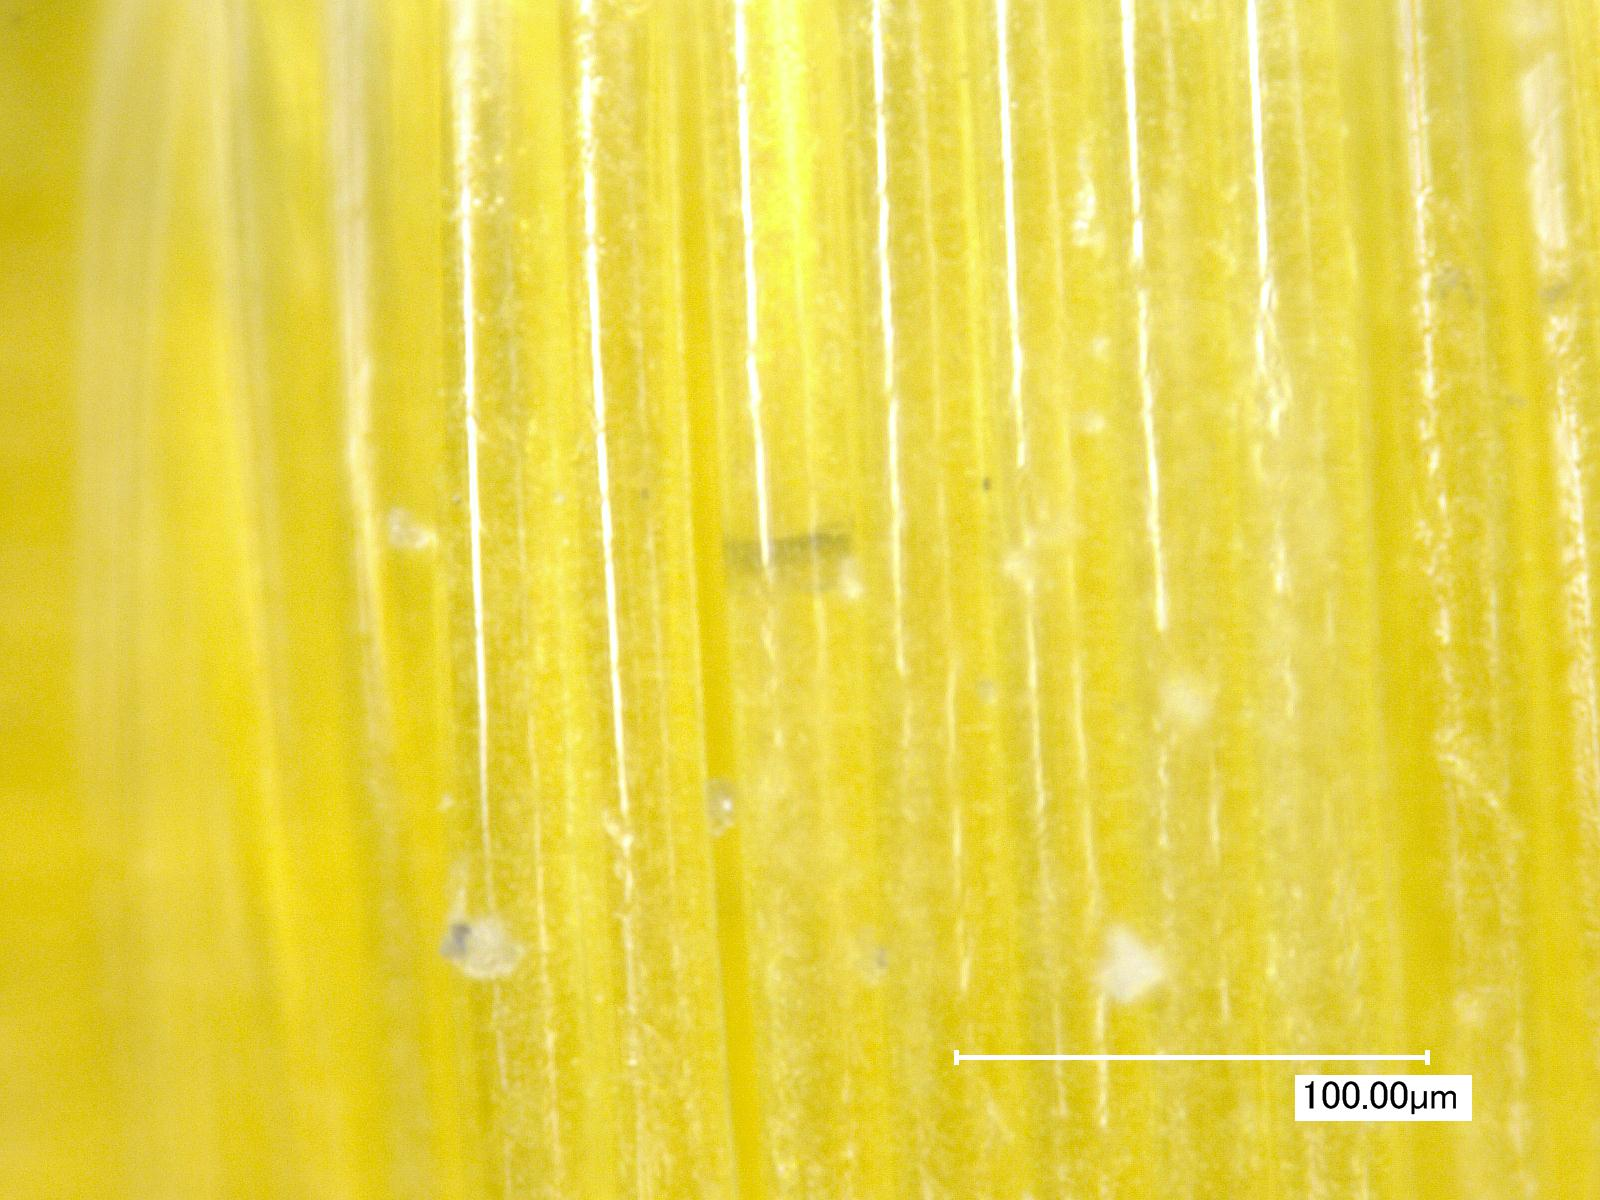
\includegraphics[keepaspectratio, width=0.8\linewidth]{figures/中心/カーリングパッド10-15.jpg}
        \caption{高倍率(1000倍)}
        \label{fig:label}
    \end{subfigure}
    \caption{10~15投使用}
    \label{fig:6}
\end{figure}

\begin{figure}[H]
    \centering
    \begin{subfigure}[htbp]{0.45\linewidth}
        \centering
        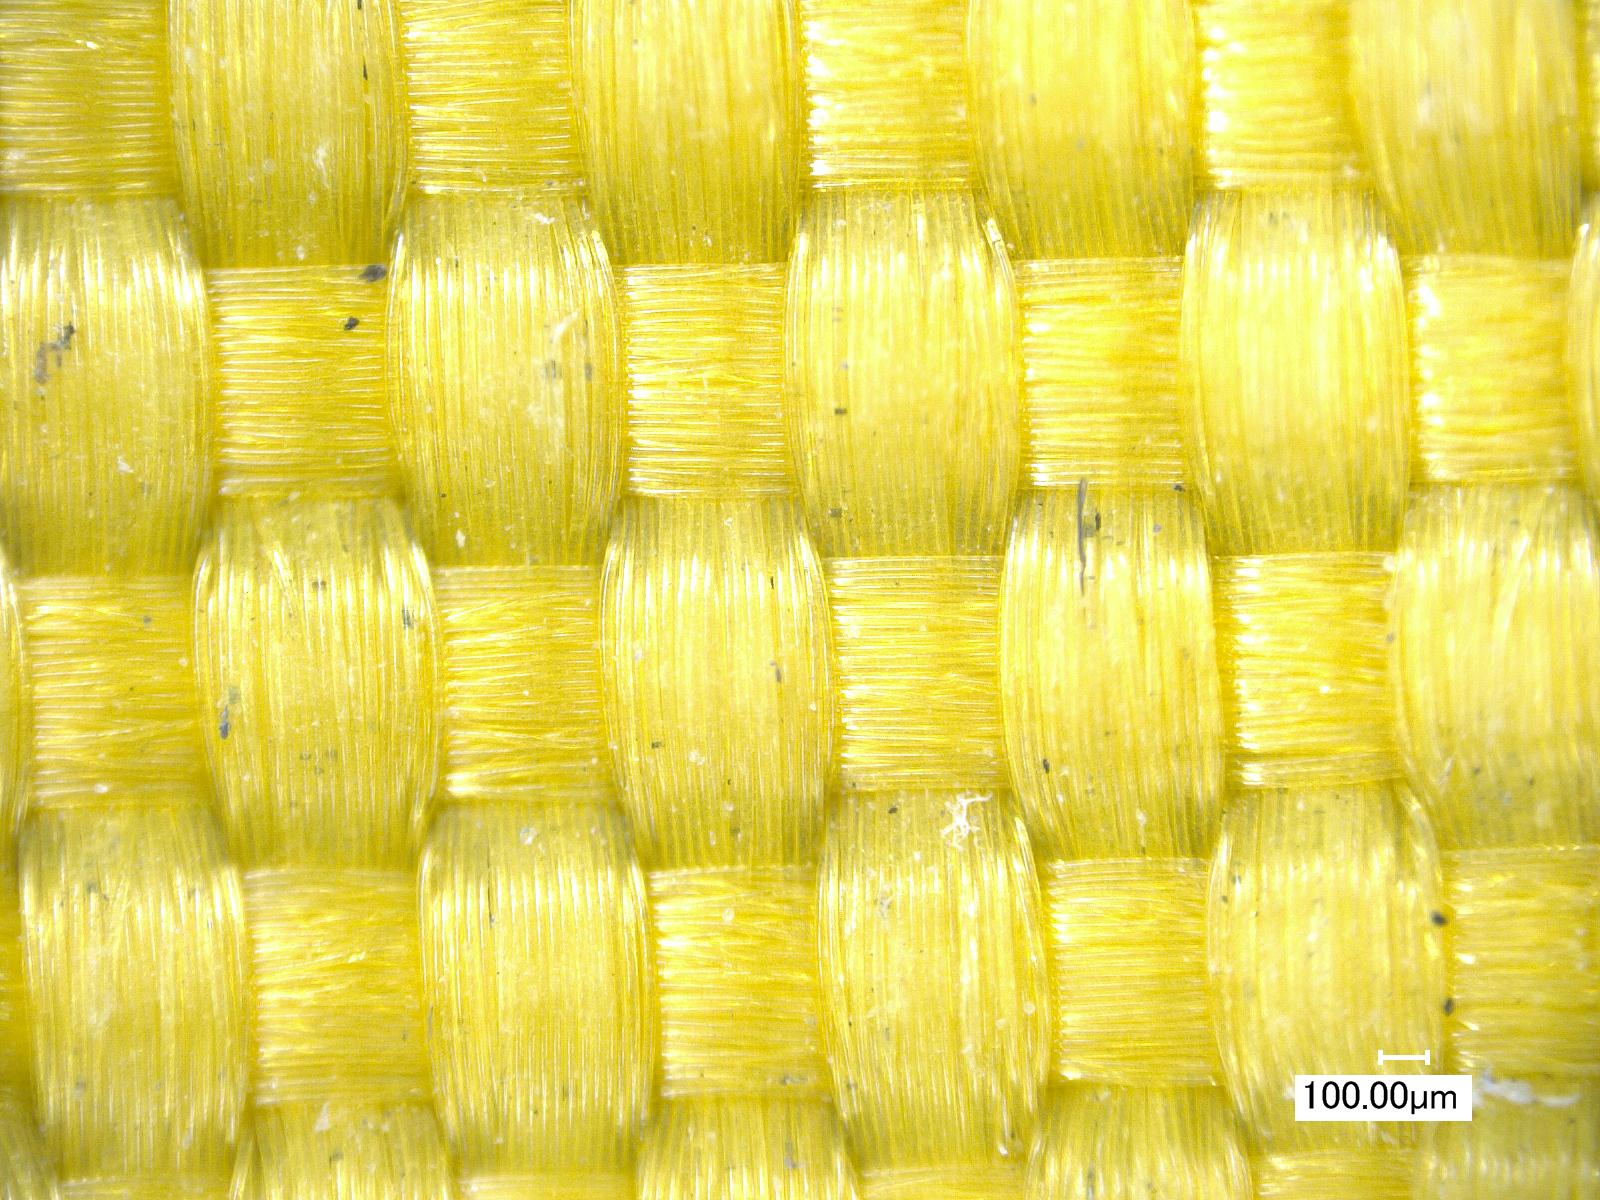
\includegraphics[keepaspectratio, width=0.8\linewidth]{figures/中心/カーリングパッド長期低倍率.jpg}
        \caption{低倍率(100倍)}
        \label{fig:label}
    \end{subfigure}
    \begin{subfigure}[htbp]{0.45\linewidth}
        \centering
        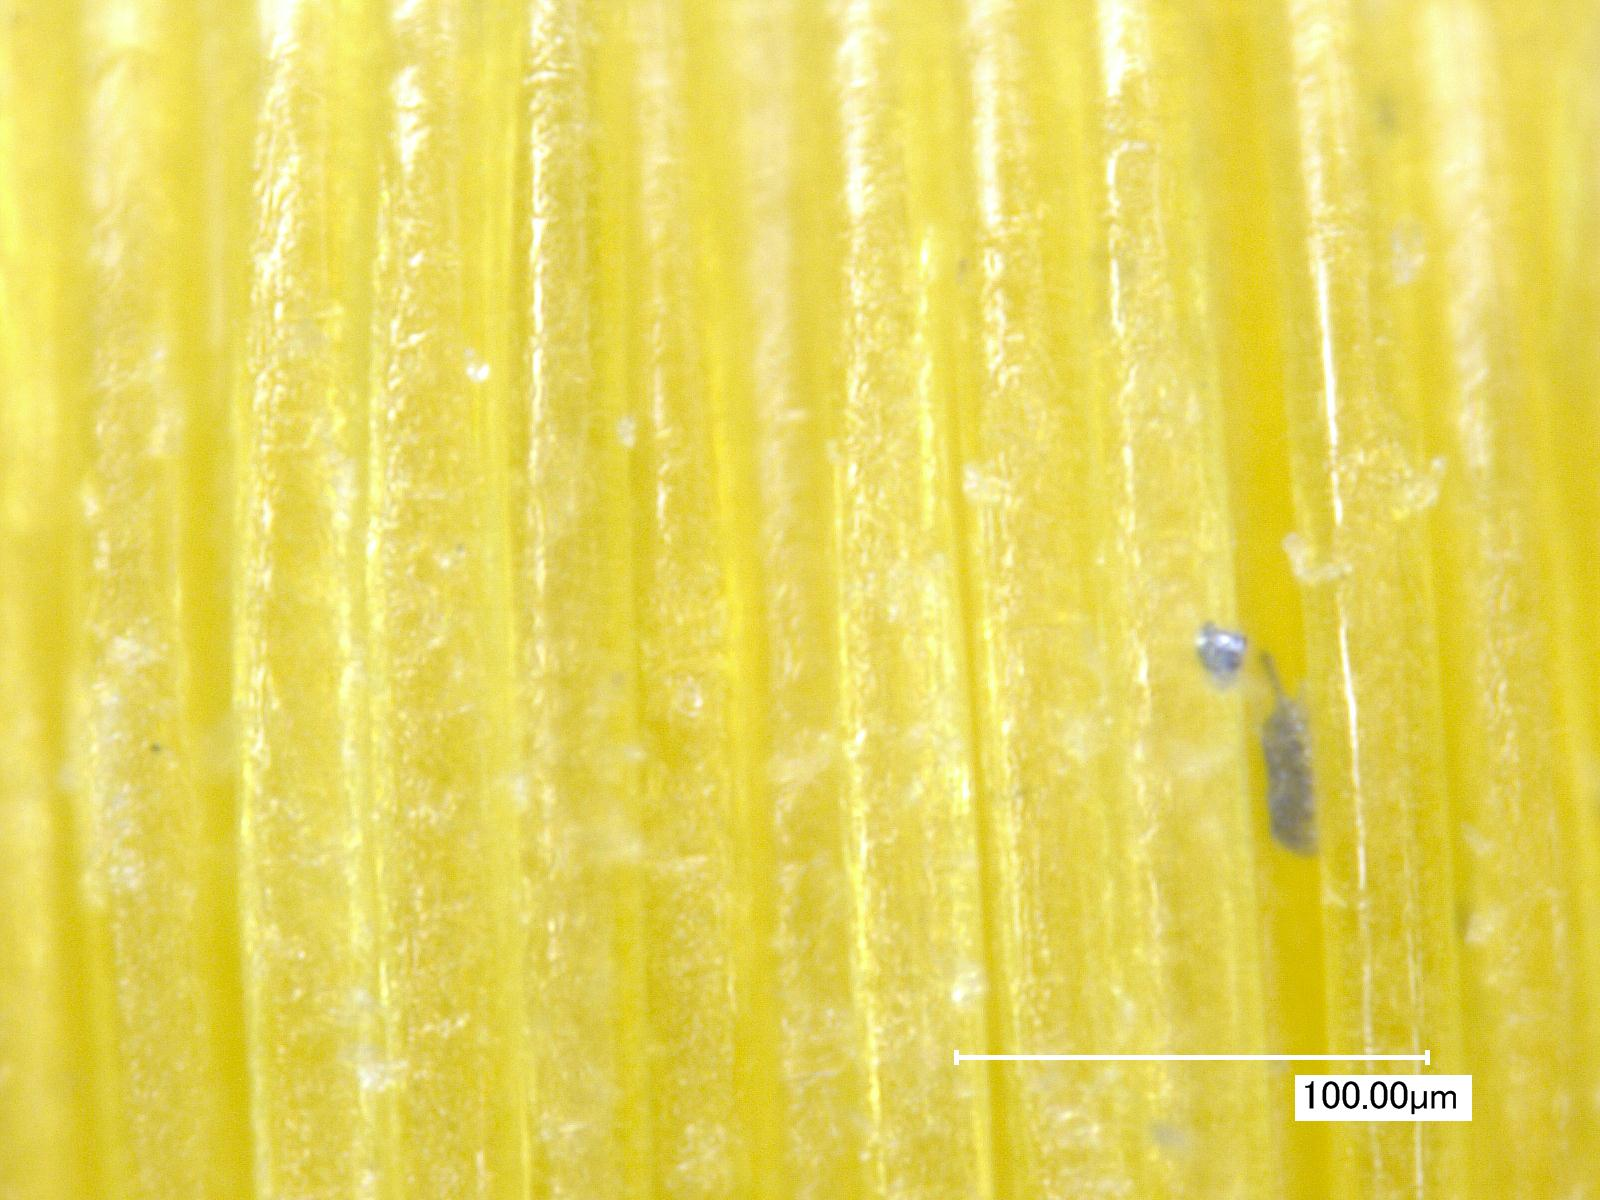
\includegraphics[keepaspectratio, width=0.8\linewidth]{figures/中心/カーリングパッド長期.jpg}
        \caption{高倍率(1000倍)}
        \label{fig:label}
    \end{subfigure}
    \caption{長期間使用}
    \label{fig:7}
\end{figure}


カーリングブラシパッドの汚れの少ない箇所は長期間使用したものでも,未使用のものと同様に,繊維が隙間なく並んでいた.
この測定結果から,カーリングブラシパッドの汚れの少ない箇所の表面繊維は,使用回数による大きな違いはなかった.

\end{document}